\documentclass[zihao=false,fontset=windows]{ctexart}
% ctexart 不接受任意 pt 选项。正文改 {10pt}，方括号里是行距。
\usepackage{scrextend}
\changefontsizes[12pt]{10pt}

\usepackage[a4paper,left=2.35cm,right=2.35cm,top=1.7cm,bottom=1.9cm]{geometry}
\usepackage{xcolor}
\usepackage{graphicx}
\usepackage{amsmath,amssymb}
\usepackage{enumitem}
\usepackage{tabularx}
\usepackage{colortbl}
\usepackage{listings}
\usepackage{hyperref}
\usepackage[most]{tcolorbox}

\definecolor{feishuText}{RGB}{31,35,41}
\definecolor{feishuBlue}{RGB}{36,91,219}
\definecolor{feishuRed}{RGB}{216,57,49}
\definecolor{feishuGray}{RGB}{100,106,115}
\definecolor{feishuGray2}{RGB}{143,149,158}
\definecolor{feishuPinkBg}{RGB}{251,191,188}
\definecolor{quoteBar}{RGB}{51,112,255}
\definecolor{codebg}{RGB}{245,246,247}
\definecolor{codeborder}{RGB}{222,224,227}
\definecolor{inlinebg}{RGB}{242,243,245}
\definecolor{callRed}{RGB}{253,226,226}
\definecolor{callOrange}{RGB}{255,245,235}
\definecolor{callYellow}{RGB}{254,255,240}
\definecolor{callGreen}{RGB}{240,251,239}
\definecolor{callBlue}{RGB}{240,244,255}
\definecolor{callRedSoft}{RGB}{254,241,241}
\definecolor{callSun}{RGB}{255,255,204}
\definecolor{tableHead}{RGB}{242,243,245}
\definecolor{tableRule}{RGB}{222,224,227}
\definecolor{codeText}{RGB}{31,35,41}
\definecolor{codeKeyword}{RGB}{0,0,255}
\definecolor{codeComment}{RGB}{0,128,0}
\definecolor{codeString}{RGB}{163,21,21}

\setmainfont{Times New Roman}
\setCJKmainfont{Microsoft YaHei}[AutoFakeBold=2.2]
\setCJKsansfont{Microsoft YaHei}[AutoFakeBold=2.2]
\setCJKmonofont{Microsoft YaHei}[AutoFakeBold=2.2]
\setmonofont{Consolas}
\newfontfamily\emojifont{Segoe UI Emoji}

\hypersetup{
  colorlinks=true,
  urlcolor=feishuBlue,
  linkcolor=feishuBlue,
  unicode=true,
  pdftitle={Qwen3-VL}
}

\setlength{\parindent}{0pt}
\setlength{\parskip}{0.42em}
\setlength{\fboxsep}{1.5pt}
\setlength{\emergencystretch}{3em}
\linespread{1.28}
\color{feishuText}
\arrayrulecolor{tableRule}
\urlstyle{same}

\setlist[enumerate]{label=\textcolor{feishuBlue}{\arabic*.}, leftmargin=1.7em, itemsep=0.22em, topsep=0.28em, parsep=0.08em, partopsep=0pt}
\setlist[itemize,1]{label=\textcolor{feishuBlue}{\textbullet}, leftmargin=1.35em, itemsep=0.18em, topsep=0.25em, parsep=0.06em, partopsep=0pt}
\setlist[itemize,2]{label=\textcolor{feishuBlue}{◦}, leftmargin=1.45em, itemsep=0.12em, topsep=0.15em}
\setlist[itemize,3]{label=\textcolor{feishuBlue}{\rule[0.18em]{0.38em}{0.38em}}, leftmargin=1.55em, itemsep=0.1em, topsep=0.12em}

\newcommand{\feiEmoji}[1]{{\emojifont #1}}
\newcommand{\incode}[1]{\colorbox{inlinebg}{\ttfamily\small #1}}
\newcommand{\bigmath}[1]{%
  \begin{center}\large$\displaystyle #1$\end{center}%
}

\lstset{
  language=Python,
  basicstyle=\ttfamily\footnotesize\color{codeText},
  keywordstyle=\color{codeKeyword},
  commentstyle=\color{codeComment},
  stringstyle=\color{codeString},
  showstringspaces=false,
  breaklines=true,
  columns=fullflexible,
  keepspaces=true,
  tabsize=4,
  upquote=true,
  aboveskip=2pt,
  belowskip=0pt,
  xleftmargin=0pt,
  frame=none
}

\tcbset{
  feishubase/.style 2 args={
    enhanced,
    boxrule=0pt,
    arc=8pt,
    left=10pt,
    right=10pt,
    top=7pt,
    bottom=7pt,
    before skip=6pt,
    after skip=6pt,
    colback=#1,
    colframe=#1,
    before upper={\feiEmoji{#2}\hspace{0.45em}\ignorespaces}
  }
}
\newtcolorbox{feishubox}[2]{feishubase={#1}{#2}, breakable}
\newtcolorbox{feishuboxnb}[2]{feishubase={#1}{#2}}

\newtcolorbox{feishuquote}{
  enhanced,
  breakable,
  boxrule=0pt,
  leftrule=3pt,
  arc=0pt,
  colframe=quoteBar,
  colback=white,
  left=8pt,
  right=2pt,
  top=2pt,
  bottom=2pt,
  before skip=4pt,
  after skip=4pt,
  before upper=\color{feishuGray}
}

\newtcolorbox{feishucode}{
  enhanced,
  breakable,
  colback=codebg,
  colframe=codeborder,
  boxrule=0.6pt,
  arc=6pt,
  left=6pt,
  right=6pt,
  top=5pt,
  bottom=4pt,
  before skip=6pt,
  after skip=6pt
}

\usepackage{needspace}
\definecolor{headRed}{RGB}{253,226,226}
\definecolor{headOrange}{RGB}{254,234,210}
\begin{document}
{\zihao{1}\bfseries Qwen3-VL\par}
\begin{feishuquote}来源：\href{https://scnajei2ds6y.feishu.cn/wiki/IBFPwd8kpiW94gkOgCIcTnDZnnh}{飞书在线文档}；复刻日期：2026年10月30日。按要求省略原文代码块。\end{feishuquote}
\begin{feishubox}{callOrange}{☘}
论文：\href{https://arxiv.org/pdf/2511.21631}{《Qwen3-VL Technical Report》}\par

代码仓库：\href{https://github.com/QwenLM/Qwen3-VL}{QwenLM/Qwen3-VL}｜完整PR代码：\href{https://github.com/huggingface/transformers/blob/088e9c30712151060aacecd3454150f4edd83cd1/src/transformers/models/qwen3_vl/modeling_qwen3_vl.py}{代码链接}｜模型仓库：\href{https://huggingface.co/collections/Qwen/qwen3-vl}{Qwen/qwen3-vl}\par

\end{feishubox}

25年9月我们在\href{https://scnajei2ds6y.feishu.cn/wiki/P8WqwpoUdicF9bkvaTqcdcS5nDb?from=from_copylink}{Qwen3 VL Preview}中超前解析了 Qwen3-VL 的模型架构，当时依靠模型代码以及 \href{https://qwenlm.github.io/blog/qwen3/}{官方Blog} 无法对模型训练细节进行解析（并且当时没有开源全系列模型）。现在随着Qwen3-VL技术报告发布/模型完整开源，我们\textcolor{feishuRed}{\textbf{重新来解析Qwen3-VL系列模型的关键技术！}}\par

Qwen3-VL是Qwen系列目前最先进的视觉-语言多模态模型（截止2025年11月），核心特性与创新：\par

\begin{itemize}[label=\textcolor{feishuBlue}{1.}]
\item \textbf{架构主要改进（对比}\textbf{\href{https://scnajei2ds6y.feishu.cn/wiki/S7Q2wviQhiYtQFk4jKvccQwDnWe}{Qwen2.5-VL}}\textbf{）}：使用的DeepStack的Projector整合多层级ViT特征提升视觉-语言对齐效果，LLM支持MoE和Dense不同架构。替换\href{https://scnajei2ds6y.feishu.cn/wiki/JboKw8o8UiaUQbk1CBDckrtFn3f}{MRoPE}为interleaved-MRoPE，强化图像/视频的时空特征建模的稳定性。

\end{itemize}

\begin{itemize}[label=\textcolor{feishuBlue}{2.}]
\item \textbf{长上下文支持}：原生支持256K tokens的长上下文，可无缝处理交错式文本、图像及视频输入。

\end{itemize}

\begin{itemize}[label=\textcolor{feishuBlue}{3.}]
\item \textbf{增强的后训练：}在多个细分领域进行RL，采用Qwen团队的SAPO，参考“think with images”多模态agent训练。

\end{itemize}

\Needspace{3cm}\par\vspace{0.9em}\begin{tcolorbox}[enhanced,colback=headRed,boxrule=0pt,arc=4pt,boxsep=0pt,left=3pt,right=3pt,top=2pt,bottom=2pt,before skip=0pt,after skip=3pt]\zihao{-2}\bfseries \textcolor{feishuBlue}{1.} 模型架构\end{tcolorbox}

\begin{feishubox}{callGreen}{☘}
模型还是标准的“三段式结构”，即 \textcolor{feishuRed}{\textbf{ViT+Projector+LLM}}：\par

\begin{itemize}[label=\textcolor{feishuBlue}{\textbullet}]
\item \textbf{Vision Encoder：}\href{https://scnajei2ds6y.feishu.cn/wiki/H3biwpNrQiAgk2kd9bscXeS2nkb}{SigLIP2}架构，初始化于SigLIP2-SO-400M、SigLIP2-Large (300M) ，进行动态分辨率CPT。沿用 Qwen2.5 bias配置、 \href{https://scnajei2ds6y.feishu.cn/wiki/BHUIwyfVUizmwQkKQPFceqJrnEe}{2D-RoPE}，但是替换了激活函数，PatchEmbed启用bias。

\end{itemize}

\begin{itemize}[label=\textcolor{feishuBlue}{\textbullet}]
\item \textbf{Projector：}Adaptor本次更新中使用了两个部分特征，一部分是沿用的Qwen2.5的 PatchMerger（对比解析参考\href{https://scnajei2ds6y.feishu.cn/wiki/KQDVwj7bAiSz8akJd3ecLLPank3}{MLLM 之 MLP Projector 发展史}）另外一部分使用了\textcolor{feishuRed}{\textbf{\incode{deepstack\_visual\_indexes}}}\textcolor{feishuRed}{\textbf{，用于与LLM跨层进行特征融合。}}

\end{itemize}

\begin{itemize}[label=\textcolor{feishuBlue}{\textbullet}]
\item \textbf{LLM：} \href{https://huggingface.co/Qwen/Qwen3-VL-235B-A22B-Instruct}{Qwen3-VL-235B-A22B} /Qwen3-VL-30B-A3B 使用的是\href{https://swfvqxo30ma.feishu.cn/wiki/Yzb0w1lKJi9EEIkeNHLcpdODnIc?from=from_copylink}{Qwen 3}的MoE版本，32B/8B/4B/2B 使用的是 Qwen3 的Dense版本，架构上使用了QKNorm（解析参考\href{https://swfvqxo30ma.feishu.cn/wiki/V2c5wrPboiCKJNkN5UocxvpLnTe?from=from_copylink}{QK Norm 的前世今生}），与\href{https://scnajei2ds6y.feishu.cn/wiki/S7Q2wviQhiYtQFk4jKvccQwDnWe}{Qwen2.5-VL}区别在于：Qwen3VL 改进了\href{https://scnajei2ds6y.feishu.cn/wiki/JboKw8o8UiaUQbk1CBDckrtFn3f}{MRoPE}为 Interleaved MRoPE。\textcolor{feishuRed}{\textbf{并且在前K层使用了DeepStack特征融合。}}

\end{itemize}

\end{feishubox}

\begin{tcbraster}[raster columns=2,raster equal height=rows,raster column skip=9pt,raster row skip=8pt]
\begin{tcolorbox}[blankest,boxrule=0pt,boxsep=0pt,left=0pt,right=0pt,top=0pt,bottom=0pt]
\begin{center}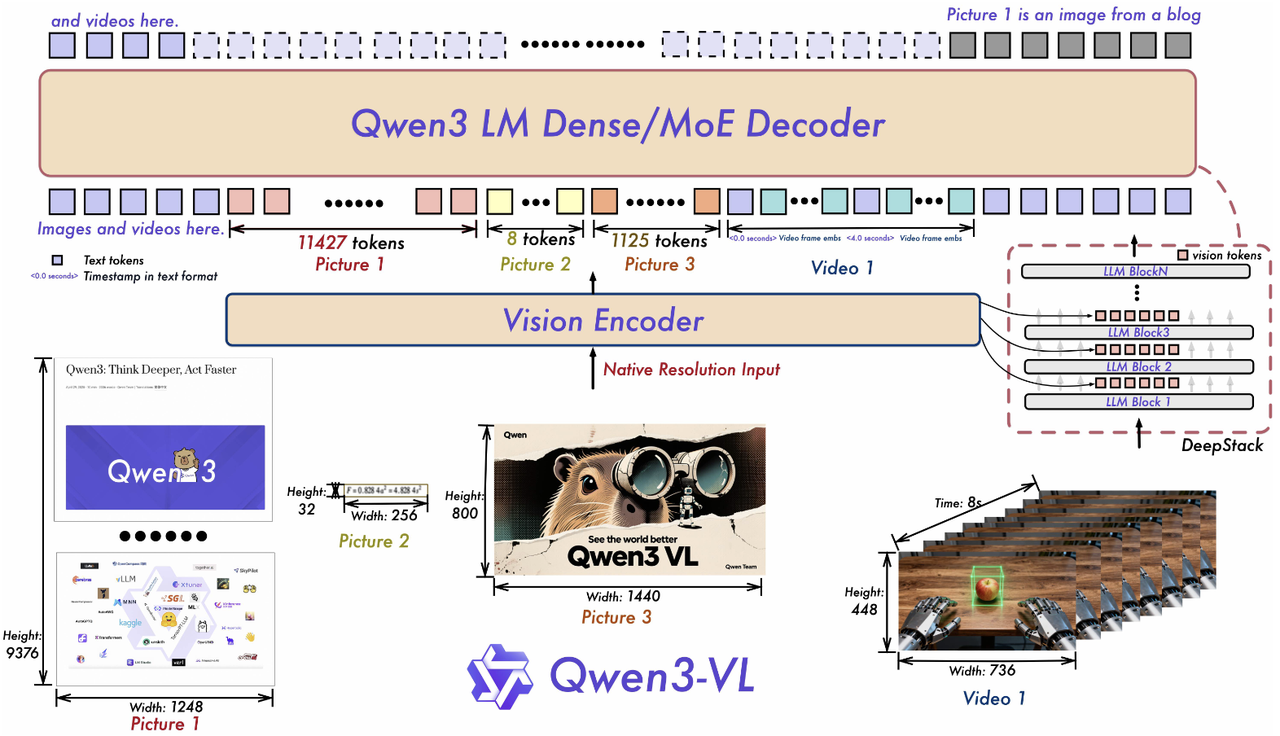
\includegraphics[width=0.98\linewidth,height=0.82\textheight,keepaspectratio]{images/Qwen3-VL/fig-01.png}\end{center}

\end{tcolorbox}
\begin{tcolorbox}[blankest,boxrule=0pt,boxsep=0pt,left=0pt,right=0pt,top=0pt,bottom=0pt]
\begin{center}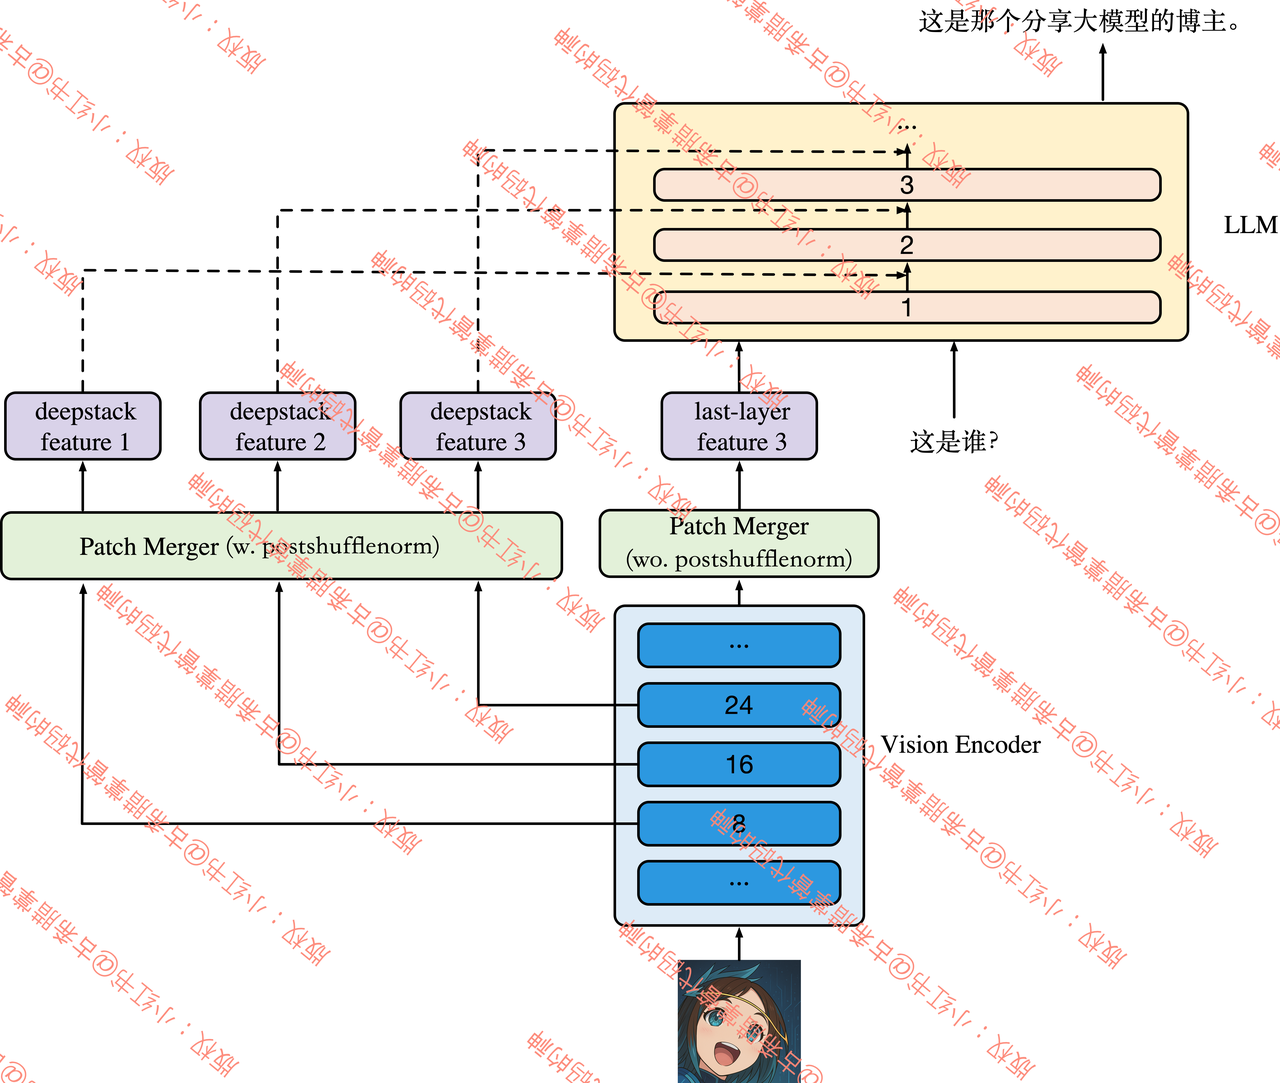
\includegraphics[width=0.98\linewidth,height=0.82\textheight,keepaspectratio]{images/Qwen3-VL/fig-02.png}\end{center}

\end{tcolorbox}
\end{tcbraster}


\Needspace{2cm}\par\vspace{0.9em}\begin{tcolorbox}[enhanced,colback=headOrange,boxrule=0pt,arc=4pt,boxsep=0pt,left=3pt,right=3pt,top=2pt,bottom=2pt,before skip=0pt,after skip=3pt]\zihao{3}\bfseries \textcolor{feishuBlue}{1.1} \textbf{Vision Encoder}\end{tcolorbox}

Vision Encoder 使用的\href{https://scnajei2ds6y.feishu.cn/wiki/H3biwpNrQiAgk2kd9bscXeS2nkb}{SigLIP2}架构，ViT权重来自于SigLIP2-SO-400M 和 SigLIP2-Large (300M) ，后者用于\textbf{2B/4B}的轻量级模型。Qwen3-VL对ViT增加 \href{https://scnajei2ds6y.feishu.cn/wiki/BHUIwyfVUizmwQkKQPFceqJrnEe}{2D-RoPE}后进行了动态分辨率的继续预训练，方法参考\href{https://arxiv.org/pdf/2503.18931}{CoMP}。对比\href{https://scnajei2ds6y.feishu.cn/wiki/S7Q2wviQhiYtQFk4jKvccQwDnWe}{Qwen2.5-VL}在ViT上的区别：\par

\begin{itemize}[label=\textcolor{feishuBlue}{\textbullet}]
\item PatchEmbed

\end{itemize}

Qwen3-VL: Qwen3VLVisionPatchEmbed 使用 Conv3d，\textcolor{feishuRed}{bias=True}， 默认 patch\_size=16。\par

Qwen2.5-VL: Qwen2\_5\_VisionPatchEmbed 也用 Conv3d，\textcolor{feishuRed}{bias=False}，默认 patch\_size=14。\par

\begin{itemize}[label=\textcolor{feishuBlue}{\textbullet}]
\item 位置编码：

\end{itemize}

两者都使用 \href{https://scnajei2ds6y.feishu.cn/wiki/BHUIwyfVUizmwQkKQPFceqJrnEe}{2D-RoPE}，即支持动态分辨率（参考\href{https://scnajei2ds6y.feishu.cn/wiki/N6PmwVkCcisDJGkC7Ypc1SfInwh}{NaViT}）。\par

\begin{itemize}[label=\textcolor{feishuBlue}{\textbullet}]
\item MLP：

\end{itemize}

之前在\href{https://scnajei2ds6y.feishu.cn/wiki/S7Q2wviQhiYtQFk4jKvccQwDnWe}{Qwen2.5-VL}中讲过，\href{https://scnajei2ds6y.feishu.cn/wiki/S7Q2wviQhiYtQFk4jKvccQwDnWe}{Qwen2.5-VL}的ViT-MLP做出了更像语言模型架构的策略：\par

\begin{itemize}[label=\textcolor{feishuBlue}{\textbullet}]
\item 使用SwiGLU的FFN结构，\incode{hidden\_act="silu"}（参考\href{https://swfvqxo30ma.feishu.cn/wiki/GkbjwrCJjiMiYwko5lfcM80Vnub}{1.1.5 前馈网络 FFN 和激活函数 Activation}）

\end{itemize}

\begin{itemize}[label=\textcolor{feishuBlue}{\textbullet}]
\item 标准化使用 RMSNorm。

\end{itemize}

\begin{itemize}[label=\textcolor{feishuBlue}{\textbullet}]
\item 其中的线性层增加bias，注意这里在llama这样的语言模型中是默认无偏置。

\end{itemize}

\textcolor{feishuRed}{\textbf{Qwen3VL 沿用了这一配置，除了激活函数：}}\par


\textcolor{feishuRed}{\textbf{但是细节变化在于激活函数由}}\textcolor{feishuRed}{\textbf{\incode{silu}}}\textcolor{feishuRed}{\textbf{替换为了}}\textcolor{feishuRed}{\textbf{\incode{gelu\_pytorch\_tanh}}}，参考代码：\par



\Needspace{2cm}\par\vspace{0.9em}\begin{tcolorbox}[enhanced,colback=headOrange,boxrule=0pt,arc=4pt,boxsep=0pt,left=3pt,right=3pt,top=2pt,bottom=2pt,before skip=0pt,after skip=3pt]\zihao{3}\bfseries \textcolor{feishuBlue}{1.1} Adaptor\end{tcolorbox}

\begin{tcbraster}[raster columns=2,raster equal height=rows,raster column skip=9pt,raster row skip=8pt]
\begin{tcolorbox}[blankest,boxrule=0pt,boxsep=0pt,left=0pt,right=0pt,top=0pt,bottom=0pt]
Adaptor在沿用了\href{https://scnajei2ds6y.feishu.cn/wiki/S7Q2wviQhiYtQFk4jKvccQwDnWe}{Qwen2.5-VL}的基础上，增加了从ViT中间层到LLM前k层到特征融合通路。总的来讲，Qwen3-VL的Adaptor包括两个部分：\par


\begin{itemize}[label=\textcolor{feishuBlue}{\textbullet}]
\item 一部分是沿用的Qwen2.5的 PatchMerger（对比解析参考\href{https://scnajei2ds6y.feishu.cn/wiki/KQDVwj7bAiSz8akJd3ecLLPank3}{MLLM 之 MLP Projector 发展史}）

\end{itemize}

\begin{itemize}[label=\textcolor{feishuBlue}{\textbullet}]
\item 另外一部分使用了\textcolor{feishuRed}{\textbf{\incode{deepstack\_visual\_indexes}}}\textcolor{feishuRed}{\textbf{，用于与LLM特征进行融合。}}如右图所示，通过特征通路进行视觉和语言的深度融合。

\end{itemize}


\end{tcolorbox}
\begin{tcolorbox}[blankest,boxrule=0pt,boxsep=0pt,left=0pt,right=0pt,top=0pt,bottom=0pt]
\begin{center}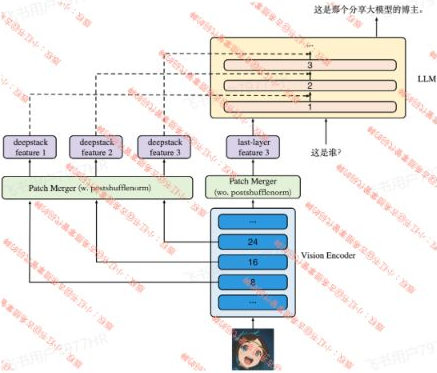
\includegraphics[width=0.98\linewidth,height=0.82\textheight,keepaspectratio]{images/Qwen3-VL/fig-03.png}\end{center}

\end{tcolorbox}
\end{tcbraster}


实现方式参考以下代码\textcolor{feishuBlue}{\textbf{蓝色}}和\textcolor{feishuRed}{\textbf{红色}}部分：\par


可以看到，\textcolor{feishuRed}{\textbf{deepstack\_merger\_list分别针对ViT的第[8, 16, 24]层设置了Qwen3VLVisionPatchMerger。}}\par

但是这部分的关键参数设置在\textcolor{feishuRed}{\textbf{use\_postshuffle\_norm}}上区别于PatchMerger，两者的关键区别在于先做shuffle（这里的shuffle本质上是hidden\_dim上进行2*2的堆叠，参考\href{https://scnajei2ds6y.feishu.cn/wiki/S7Q2wviQhiYtQFk4jKvccQwDnWe}{Qwen2.5-VL}）还是先做LayerNorm：\par


然后整体上看，Qwen3VLVisionModel（即ViT部分），提供给LLM的是两部分特征：\par

\begin{itemize}[label=\textcolor{feishuBlue}{\textbullet}]
\item hidden\_states：最后一层通过PatchMerger的特征。

\end{itemize}

\begin{itemize}[label=\textcolor{feishuBlue}{\textbullet}]
\item \textcolor{feishuRed}{\textbf{deepstack\_feature\_lists：第[8, 16, 24]层中间特征。}}

\end{itemize}

代码参考，具体这两部分特征怎么用，我们看LLM部分代码：\par


至于为什么要用中间特征，参考：\href{https://scnajei2ds6y.feishu.cn/wiki/ORZvwHCgti5VehknsbRcLCYTnuh\#share-YCPndVmp9oTL5Dxct5xcxYQTn1e}{多模态LLM中adapter部分的设计，ViT的特征取哪层哪个位置？（字节-2面）}\par


\Needspace{2cm}\par\vspace{0.9em}\begin{tcolorbox}[enhanced,colback=headOrange,boxrule=0pt,arc=4pt,boxsep=0pt,left=3pt,right=3pt,top=2pt,bottom=2pt,before skip=0pt,after skip=3pt]\zihao{3}\bfseries \textcolor{feishuBlue}{1.2} LLM\end{tcolorbox}

分为\href{https://swfvqxo30ma.feishu.cn/wiki/Yzb0w1lKJi9EEIkeNHLcpdODnIc?from=from_copylink}{Qwen 3}的MoE版本/非MoE版本，具体开源的模型版本和LLM架构见表：\par

\begin{center}\begin{tabularx}{\linewidth}{|p{0.2\linewidth}|X|}\hline
\rowcolor{tableHead} 规格（架构）\par
 & 模型名字\par
 \\ \hline
\textbf{235B (MoE)}\par
 & Qwen3-VL-235B-A22B-Instruct / Thinking / FP8 / GGUF\par
 \\ \hline
\textbf{30B (MoE)}\par
 & Qwen3-VL-30B-A3B-Instruct / Thinking / FP8 / GGUF\par
 \\ \hline
\textbf{32B (Dense)}\par
 & Qwen3-VL-32B-Instruct / Thinking / FP8 / GGUF\par
 \\ \hline
\textbf{8B (Dense)}\par
 & Qwen3-VL-8B-Instruct / Thinking / FP8 / GGUF\par
 \\ \hline
\textbf{4B (Dense)}\par
 & Qwen3-VL-4B-Instruct / Thinking / FP8 / GGUF\par
 \\ \hline
\textbf{2B (Dense)}\par
 & Qwen3-VL-2B-Instruct / Thinking / FP8 / GGUF\par
 \\ \hline
\end{tabularx}\end{center}

架构上使用了QKNorm（解析参考\href{https://swfvqxo30ma.feishu.cn/wiki/V2c5wrPboiCKJNkN5UocxvpLnTe?from=from_copylink}{QK Norm 的前世今生}），对于非MoE版本进行分析，区别在于：\par

\begin{itemize}[label=\textcolor{feishuBlue}{\textbullet}]
\item Qwen3VL 使用 3 维多模态位置编码 \href{https://scnajei2ds6y.feishu.cn/wiki/JboKw8o8UiaUQbk1CBDckrtFn3f}{MRoPE} ，Qwen3 则使用标准 RoPE。

\end{itemize}

\begin{itemize}[label=\textcolor{feishuBlue}{\textbullet}]
\item Qwen3 支持 sliding window 层，Qwen3VL 未引入。

\end{itemize}

\begin{itemize}[label=\textcolor{feishuBlue}{\textbullet}]
\item \textcolor{feishuRed}{\textbf{在前K层使用了DeepStack特征融合。（详细参考 }}\textcolor{feishuRed}{\href{https://w0rg9.xetlk.com/s/17bFhM}{Qwen3-VL的 DeepStack 技术是什么？}}\textcolor{feishuRed}{\textbf{）}}

\end{itemize}

我们具体来看，ViT输出的特征如何与LLM特征进行融合的，首先ViT输出的特征是两部分：\par

\begin{itemize}[label=\textcolor{feishuBlue}{\textbullet}]
\item hidden\_states：最后一层通过PatchMerger的特征。

\end{itemize}

\begin{itemize}[label=\textcolor{feishuBlue}{\textbullet}]
\item \textcolor{feishuRed}{\textbf{deepstack\_feature\_lists：第[8, 16, 24]层中间特征。}}

\end{itemize}

首先对于hidden\_states，直接与文本特征拼接输入LLM：\par


\begin{tcbraster}[raster columns=2,raster equal height=rows,raster column skip=9pt,raster row skip=8pt]
\begin{tcolorbox}[blankest,boxrule=0pt,boxsep=0pt,left=0pt,right=0pt,top=0pt,bottom=0pt]
然后对于\textcolor{feishuRed}{\textbf{deepstack\_feature\_lists，则是分别与前K层（这里是前三层，}}\textcolor{feishuRed}{\textbf{\incode{K=len(deepstack\_feature\_lists)}}}\textcolor{feishuRed}{\textbf{）进行融合。}}\par


我们首先来看这部分融合的代码逻辑：\par

\end{tcolorbox}
\begin{tcolorbox}[blankest,boxrule=0pt,boxsep=0pt,left=0pt,right=0pt,top=0pt,bottom=0pt]
\begin{center}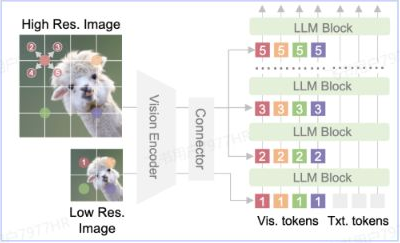
\includegraphics[width=0.98\linewidth,height=0.82\textheight,keepaspectratio]{images/Qwen3-VL/fig-04.png}\end{center}

\end{tcolorbox}
\end{tcbraster}


然后融合的方式参考\_deepstack\_process函数，具体处理逻辑为：\par

\begin{itemize}[label=\textcolor{feishuBlue}{\textbullet}]
\item 把 hidden\_states 在 visual\_pos\_masks 为 True 的位置切出来，加上对应层的视觉特征向量 visual\_embeds（就是 deepstack\_visual\_embeds[layer\_idx]，它已经对齐到“\textcolor{feishuRed}{\textbf{只有视觉位置}}”的子序列顺序）。

\end{itemize}

\begin{itemize}[label=\textcolor{feishuBlue}{\textbullet}]
\item 再写回到 hidden\_states 的这些视觉位置。

\end{itemize}

这等价于：在若干前层（deepstack 的层数）里，用视觉中间层特征对语言隐藏态进行残差式强制注入，\textcolor{feishuRed}{\textbf{仅作用于视觉 token 的那些位置，文本 token 位置不变：}}\par



\Needspace{2cm}\par\vspace{0.9em}\noindent{\zihao{4}\bfseries \textcolor{feishuBlue}{1.2.1} Interleaved MRoPE}\par\vspace{0.28em}

鹅圈子有详细解析，麻烦查看：\href{https://appttaswqlt5080.h5.xet.citv.cn/xe.community.community_service/v2/feedDetail?app_id=appttaswqlt5080&community_id=c_68afda70f9bc6_x29igT7o2026&feed_id=d_693f158d4bd48_CMsdjT4h3woi&share_user_id=&share_type=}{链接}\par


\Needspace{6cm}\par\vspace{0.9em}\begin{tcolorbox}[enhanced,colback=headRed,boxrule=0pt,arc=4pt,boxsep=0pt,left=3pt,right=3pt,top=2pt,bottom=2pt,before skip=0pt,after skip=3pt]\zihao{-2}\bfseries \textcolor{feishuBlue}{2.} 预训练\end{tcolorbox}

\Needspace{2cm}\par\vspace{0.9em}\begin{tcolorbox}[enhanced,colback=headOrange,boxrule=0pt,arc=4pt,boxsep=0pt,left=3pt,right=3pt,top=2pt,bottom=2pt,before skip=0pt,after skip=3pt]\zihao{3}\bfseries \textcolor{feishuBlue}{2.1} 训练配置\end{tcolorbox}

\begin{center}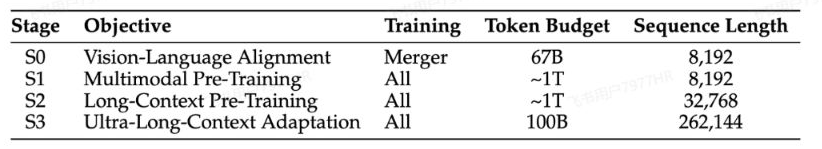
\includegraphics[width=0.98\linewidth,height=0.82\textheight,keepaspectratio]{images/Qwen3-VL/fig-05.png}\end{center}

\textcolor{feishuRed}{\textbf{首先在S0之前需要对ViT进行CPT（继续预训练），主要目标是拓展其在动态分辨率下的能力，这部分不算在Stage里面。}}\par

\begin{itemize}[label=\textcolor{feishuBlue}{1.}]
\item \textbf{Stage-0：视觉-语言对齐}

\end{itemize}

\begin{itemize}[label=\textcolor{feishuBlue}{\textbullet}]
\item 目标：视觉与语言模态对齐

\end{itemize}

\begin{itemize}[label=\textcolor{feishuBlue}{\textbullet}]
\item 方法：\textcolor{feishuRed}{仅训练MLP融合器}，视觉编码器和LLM冻结

\end{itemize}

\begin{itemize}[label=\textcolor{feishuBlue}{\textbullet}]
\item 数据：67B tokens（高质量图文对、OCR、世界知识）

\end{itemize}

\begin{itemize}[label=\textcolor{feishuBlue}{2.}]
\item \textbf{Stage-1：多模态预训练}

\end{itemize}

\begin{itemize}[label=\textcolor{feishuBlue}{\textbullet}]
\item 目标：全参数端到端训练

\end{itemize}

\begin{itemize}[label=\textcolor{feishuBlue}{\textbullet}]
\item 方法：全参数训练，混合视觉Instruction数据与纯文本数据

\end{itemize}

\begin{itemize}[label=\textcolor{feishuBlue}{\textbullet}]
\item 数据：\textasciitilde{}1T tokens（含交错图文、视觉定位、VQA、STEM数据及少量视频）

\end{itemize}

\begin{itemize}[label=\textcolor{feishuBlue}{3.}]
\item \textbf{Stage-2：长上下文预训练}

\end{itemize}

\begin{itemize}[label=\textcolor{feishuBlue}{\textbullet}]
\item 目标：扩展上下文处理能力

\end{itemize}

\begin{itemize}[label=\textcolor{feishuBlue}{\textbullet}]
\item 调整：序列长度增至32768，增加纯文本比例和视频/任务数据

\end{itemize}

\begin{itemize}[label=\textcolor{feishuBlue}{\textbullet}]
\item 数据：\textasciitilde{}1T tokens（强化长视频与多步骤任务理解）

\end{itemize}

\begin{itemize}[label=\textcolor{feishuBlue}{4.}]
\item \textbf{Stage-3：超长上下文适应}

\end{itemize}

\begin{itemize}[label=\textcolor{feishuBlue}{\textbullet}]
\item 目标：突破上下文窗口极限

\end{itemize}

\begin{itemize}[label=\textcolor{feishuBlue}{\textbullet}]
\item 调整：序列长度扩展至262144

\end{itemize}

\begin{itemize}[label=\textcolor{feishuBlue}{\textbullet}]
\item 数据：100B tokens（聚焦长视频/长文档分析任务）

\end{itemize}

\Needspace{2cm}\par\vspace{0.9em}\begin{tcolorbox}[enhanced,colback=headOrange,boxrule=0pt,arc=4pt,boxsep=0pt,left=3pt,right=3pt,top=2pt,bottom=2pt,before skip=0pt,after skip=3pt]\zihao{3}\bfseries \textcolor{feishuBlue}{2.2} 数据来源\end{tcolorbox}

\begin{feishubox}{callBlue}{☘}
\textbf{数据合成方法论}：\par

1）强调模型标注（Qwen2.5VL系列）的数据合成、过滤与验证。\par

2）合成数据与真实数据配比、多样性采样，平衡规模与质量。\par

3）多阶段处理流程（生成$\rightarrow$验证），确保数据可靠性。\par

4）统一标注框架与标准化设计（如坐标、格式）提升泛化性。\par

\end{feishubox}

\begin{itemize}[label=\textcolor{feishuBlue}{\textbullet}]
\item \textbf{图像-文本对数据（Image-Caption Pairs）}

\end{itemize}

使用\href{https://scnajei2ds6y.feishu.cn/wiki/S7Q2wviQhiYtQFk4jKvccQwDnWe}{Qwen2.5-VL}-32B模型对原始文本进行重新标注，生成更细粒度的描述（对象属性、空间布局等）。\par

基于视觉嵌入的聚类增强，对数据分布稀疏区域并进行定向增强。\par

\begin{itemize}[label=\textcolor{feishuBlue}{\textbullet}]
\item \textbf{交错文本-图像数据（Interleaved Text-Image）}

\end{itemize}

对（多模态）网页、书籍使用\href{https://scnajei2ds6y.feishu.cn/wiki/S7Q2wviQhiYtQFk4jKvccQwDnWe}{Qwen2.5-VL}-7B（轻量级模型）进行多模态解析，精确对齐文本与图表/照片。\par

低价值内容过滤：移除纯文本/未对齐片段，要求最低页面数、图像-文本比例。\par

最终需要切分、合并为最长不超过256K token的序列。\par

\begin{itemize}[label=\textcolor{feishuBlue}{\textbullet}]
\item \textbf{知识实体数据（World Knowledge）}

\end{itemize}

百科数据，覆盖10+语义类别（动物/植物/地标等）。\par

重要性采样策略：高显著性实体高频采样，低显著性实体低频保留。\par

使用LLM生成增强描述，包含视觉属性、空间关系和交互信息。\par

\begin{itemize}[label=\textcolor{feishuBlue}{\textbullet}]
\item \textbf{OCR与文档解析}

\end{itemize}

OCR：30M内部样本 + 30M合成多语言样本，均使用Qwen2.5-VL标注。\par

文档解析：3M PDF + 4M内部文档，使用布局模型预测阅读顺序，Qwen2.5-VL-72B进行区域识别（类似\href{https://scnajei2ds6y.feishu.cn/wiki/CmMSw5yIki7NTckgkg7cayIxnWc}{PaddleOCR-VL}）。\par

\begin{itemize}[label=\textcolor{feishuBlue}{\textbullet}]
\item \textbf{视觉定位与计数（Grounding and Counting）}

\end{itemize}

融合开源数据与合成数据构建框/点定位数据集，通过\href{https://scnajei2ds6y.feishu.cn/wiki/S7Q2wviQhiYtQFk4jKvccQwDnWe}{Qwen2.5-VL}进行标注/低置信度过滤。\par

计数任务涵盖直接计数、先给出框/点再引导计数、[0,1000]先坐标标准化后再计数三种形式。\par

\begin{itemize}[label=\textcolor{feishuBlue}{\textbullet}]
\item \textcolor{feishuRed}{\textbf{空间与3D理解（Spatial Understanding and 3D Recognition）}}

\end{itemize}

相比视觉定位与计数，3D理解需要推理空间关系、功能推断（如“可抓握”“可按压”）以及可行动作序列（如“如何移动障碍物拿到书”），目标是为具身智能（Embodied AI）和交互系统提供基础，支持对3D场景的深层语义理解。\par

空间理解数据合成：融合真实场景与合成布局数据，通过模板和LLM生成多样化自然语言查询，强调相对空间关系表达（非绝对坐标）。\par

3D定位数据合成：整合多源公共场景数据，构建单目图像+自然语言指代+3D边界框（9自由度）的问答格式数据集。过滤遮挡/噪声标签，统一至虚拟相机坐标系（基于Omni3D方法），确保空间一致性。合成细粒度描述文本，涵盖物体属性、布局、空间位置及交互关系，提升指代表达精准度。\par

\begin{itemize}[label=\textcolor{feishuBlue}{\textbullet}]
\item \textbf{多模态代码能力（Code）}

\end{itemize}

复用Qwen3-Coder系列大规模代码语料。\par

开源整理+合成多模态Coding数据集：UI转HTML/CSS、SVG生成、流程图转代码等。\par

\begin{itemize}[label=\textcolor{feishuBlue}{\textbullet}]
\item \textbf{视频理解（Video）}

\end{itemize}

在视频数据集的内容多样性上进行均衡采样。\par

FPS动态采样策略：根据序列长度约束调整fps和最大帧数。\par

利用字幕模型进行密集标注，合成时间连贯的 caption label。\par

\begin{itemize}[label=\textcolor{feishuBlue}{\textbullet}]
\item \textbf{STEM多模态推理（Science, Technology, Engineering, and Mathematics）}

\end{itemize}

使用代码生成图示的方法生成几何图表数据：1M点标注样本 + 2M视觉问答对，并使用reward model进行检查。\par

多模态推理：60M K-12/本科习题 + 12M合成推理样本，通过\textcolor{feishuRed}{拒绝采样}仅保留具有挑战性的问题。\par

\begin{itemize}[label=\textcolor{feishuBlue}{\textbullet}]
\item \textcolor{feishuRed}{\textbf{代理数据（Agent）}}

\end{itemize}

GUI交互数据涵盖跨平台界面感知与多步任务轨迹：在跨平台界面感知方面，通过元数据、解析工具和人工标注构建了诸如元素描述、密集字幕生成和密集定位等任务，从而实现对多样化用户界面的稳健理解。在多步任务方面，通过一个自我演化的轨迹生成框架组装多步骤任务轨迹，并辅以针对性的人工审核。\par

函数调用通过合成Pipeline实现无需真实执行的数据合成：首先通过图像指导\textcolor{feishuRed}{具备能力的模型}生成用户查询及其对应的功能定义。接着我们采样模型的功能调用并生成其推理过程，并合成功能响应。该过程会不断重复，直到用户的查询被判断为已解决，剔除其中格式错误的轨迹。\par

搜索能力集成在线工具，支持长尾实体知识获取：通过在线图像搜索和文本搜索工具收集多模态事实查询轨迹，鼓励模型对不熟悉的实体进行搜索。通过这种方式，模型学会了从网络上收集信息，从而生成更加准确的响应。\par


\Needspace{3cm}\par\vspace{0.9em}\begin{tcolorbox}[enhanced,colback=headRed,boxrule=0pt,arc=4pt,boxsep=0pt,left=3pt,right=3pt,top=2pt,bottom=2pt,before skip=0pt,after skip=3pt]\zihao{-2}\bfseries \textcolor{feishuBlue}{3.} 后训练\end{tcolorbox}

后训练流程分为三个阶段，旨在提升模型的指令遵循、推理能力及人类偏好对齐：\par

\textbf{Stage 1：监督微调（SFT）}\par

\begin{itemize}[label=\textcolor{feishuBlue}{\textbullet}]
\item 目标：激活指令遵循能力与潜在推理技能。

\end{itemize}

\begin{itemize}[label=\textcolor{feishuBlue}{\textbullet}]
\item 实现方式：
\begin{itemize}[label=\textcolor{feishuBlue}{\textbullet}]
\item 两阶段训练：
\begin{itemize}[label=\textcolor{feishuBlue}{i.}]
\item 初始阶段：基于32k上下文长度进行训练。

\end{itemize}

\begin{itemize}[label=\textcolor{feishuBlue}{ii.}]
\item 扩展阶段：将上下文窗口扩展至256k，专注于长文档和长视频数据的处理。

\end{itemize}

\end{itemize}

\begin{itemize}[label=\textcolor{feishuBlue}{\textbullet}]
\item 数据分类：
\begin{itemize}[label=\textcolor{feishuBlue}{\textbullet}]
\item 标准格式：适用于非思考模型（Instruct模型）。

\end{itemize}

\begin{itemize}[label=\textcolor{feishuBlue}{\textbullet}]
\item 思维链（CoT）格式：显式建模推理过程，适用于思考模型（Thinking模型）。

\end{itemize}

\end{itemize}

\end{itemize}

\textbf{Stage 2：强到弱蒸馏（Strong-to-Weak Distillation）}\par

\begin{itemize}[label=\textcolor{feishuBlue}{\textbullet}]
\item 核心方法：通过知识蒸馏，将强教师模型的能力迁移至学生模型。

\end{itemize}

\begin{itemize}[label=\textcolor{feishuBlue}{\textbullet}]
\item 关键设计：
\begin{itemize}[label=\textcolor{feishuBlue}{\textbullet}]
\item 纯文本数据微调：仅使用\textcolor{feishuRed}{纯文本数据}对LLM主干进行优化。

\end{itemize}

\begin{itemize}[label=\textcolor{feishuBlue}{\textbullet}]
\item 效果：显著提升文本任务与多模态任务的推理能力。

\end{itemize}

\end{itemize}

\textbf{Stage 3：强化学习（RL）}\par

\begin{itemize}[label=\textcolor{feishuBlue}{\textbullet}]
\item 目标：增强模型性能与人类偏好对齐，优化细粒度能力。

\end{itemize}

\begin{itemize}[label=\textcolor{feishuBlue}{\textbullet}]
\item 子阶段划分：
\begin{itemize}[label=\textcolor{feishuBlue}{\textbullet}]
\item 推理RL：针对数学、OCR、基础推理等需逻辑推导的领域。

\end{itemize}

\begin{itemize}[label=\textcolor{feishuBlue}{\textbullet}]
\item 通用RL：覆盖多模态任务（如指令遵循、文本-图像对齐等）。

\end{itemize}

\end{itemize}

\Needspace{2cm}\par\vspace{0.9em}\begin{tcolorbox}[enhanced,colback=headOrange,boxrule=0pt,arc=4pt,boxsep=0pt,left=3pt,right=3pt,top=2pt,bottom=2pt,before skip=0pt,after skip=3pt]\zihao{3}\bfseries \textcolor{feishuBlue}{3.1} SFT\end{tcolorbox}

这部分方法是确定的，就是做Instruction Tuning。关键在于数据构建，分为两个部分：Instruct模型（非思考模型）数据构建、Thinking模型（思考模型）数据构建。\par

\Needspace{2cm}\par\vspace{0.9em}\noindent{\zihao{4}\bfseries \textcolor{feishuRed}{\textbf{Instruct 模型SFT数据}}}\par\vspace{0.28em}

在\href{https://scnajei2ds6y.feishu.cn/wiki/S7Q2wviQhiYtQFk4jKvccQwDnWe}{Qwen2.5-VL}的8大核心领域、30个类别基础上进行拓展，新增空间推理（具身智能）、细粒度视觉理解、视频时空定位（目标追踪）及长上下文技术文档解析等类别的数据。\par

\begin{itemize}[label=\textcolor{feishuBlue}{\textbullet}]
\item \textbf{数据规模与组成}：SFT数据集包含约120万样本，其中：
\begin{itemize}[label=\textcolor{feishuBlue}{\textbullet}]
\item \textbf{单模态数据}（1/3）：纯文本数据条目。

\end{itemize}

\begin{itemize}[label=\textcolor{feishuBlue}{\textbullet}]
\item \textbf{多模态数据}（2/3）：图像-文本对、视频-文本对，支持复杂场景解析。

\end{itemize}

\end{itemize}

\begin{itemize}[label=\textcolor{feishuBlue}{\textbullet}]
\item \textbf{分阶段训练}：为适配256K token长上下文能力，采用两阶段训练：
\begin{itemize}[label=\textcolor{feishuBlue}{\textbullet}]
\item \textbf{第一阶段}：32K token序列长度，训练1个epoch；

\end{itemize}

\begin{itemize}[label=\textcolor{feishuBlue}{\textbullet}]
\item \textbf{第二阶段}：256K token全长度，混合长上下文数据与32K token样本（\textcolor{feishuRed}{采用课程学习策略}）。

\end{itemize}

\end{itemize}

采用 \textbf{两阶段过滤 }对查询（query）和响应（response）进行过滤，一方面需要保证查询足够清晰、可验证。另外一方面需要保证响应正确、无害。\par

\begin{itemize}[label=\textcolor{feishuBlue}{\textbullet}]
\item \textbf{查询过滤}：
\begin{itemize}[label=\textcolor{feishuBlue}{\textbullet}]
\item 使用\textcolor{feishuRed}{Qwen2.5-VL过滤}不可验证或模糊指令。

\end{itemize}

\begin{itemize}[label=\textcolor{feishuBlue}{\textbullet}]
\item 修订歧义查询，保留语义意图。

\end{itemize}

\begin{itemize}[label=\textcolor{feishuBlue}{\textbullet}]
\item 剔除低信息密度网络查询，保留高复杂度、高相关性样本。

\end{itemize}

\end{itemize}

\begin{itemize}[label=\textcolor{feishuBlue}{\textbullet}]
\item \textbf{响应过滤}：
\begin{itemize}[label=\textcolor{feishuBlue}{\textbullet}]
\item \textbf{规则过滤（Rule-Based Filtering）}：去除重复、不完整、格式错误或有害内容。

\end{itemize}

\begin{itemize}[label=\textcolor{feishuBlue}{\textbullet}]
\item \textbf{模型过滤（Model-Based Filtering）}：基于Qwen2.5-VL的奖励模型多维度评估。
\begin{itemize}[label=\textcolor{feishuBlue}{\textbullet}]
\item \textbf{答案质量}：正确性、完整性、清晰度、实用性。

\end{itemize}

\begin{itemize}[label=\textcolor{feishuBlue}{\textbullet}]
\item \textbf{视觉任务}：重点验证视觉信息利用的准确性。

\end{itemize}

\begin{itemize}[label=\textcolor{feishuBlue}{\textbullet}]
\item \textbf{隐蔽问题检测}：识别语言混杂、风格突变等规则难以覆盖的缺陷。

\end{itemize}

\end{itemize}

\end{itemize}

\textcolor{feishuRed}{\textbf{思考模型 Long-CoT 冷启动数据}}\par

为了对Thinking模型进行冷启动SFT，构建专门的长思维链（Long-CoT）冷启动数据集，其中多模态与纯文本数据1:1混合：\par

\begin{itemize}[label=\textcolor{feishuBlue}{1.}]
\item \textbf{数据构成}
\begin{itemize}[label=\textcolor{feishuBlue}{\textbullet}]
\item 多模态数据（占比50\%）：聚焦视觉问答（VQA）、OCR、2D/3D定位、视频分析等传统任务，强化STEM与智能体工作流相关的高阶推理能力。

\end{itemize}

\begin{itemize}[label=\textcolor{feishuBlue}{\textbullet}]
\item 纯文本数据（占比50\%）：延续Qwen3的数据特征，覆盖数学、代码生成、逻辑推理等复杂学科领域。

\end{itemize}

\end{itemize}

\begin{itemize}[label=\textcolor{feishuBlue}{2.}]
\item \textbf{过滤低质、简单样本方法}
\begin{itemize}[label=\textcolor{feishuBlue}{\textbullet}]
\item \textbf{难度校准}：我们选择性地保留基线模型通过率较低或生成较长、更详细回复的实例。这使得数据集中包含了对当前模型而言真正具有挑战性的问题。

\end{itemize}

\begin{itemize}[label=\textcolor{feishuBlue}{\textbullet}]
\item \textbf{多模态必要性筛选}：通过Qwen3-30B-nothink模型过滤可仅凭文本解决的视觉数学问题，保证视觉输入的必要性。

\end{itemize}

\begin{itemize}[label=\textcolor{feishuBlue}{\textbullet}]
\item \textbf{响应净化机制}：
\begin{itemize}[label=\textcolor{feishuBlue}{\textbullet}]
\item 答案核对：优先剔除含错误答案的候选答案。

\end{itemize}

\begin{itemize}[label=\textcolor{feishuBlue}{\textbullet}]
\item 过程核对：二次过滤存在重复表达、语言混杂、缺乏逻辑推演的猜测型回答。

\end{itemize}

\end{itemize}

\end{itemize}

\Needspace{2cm}\par\vspace{0.9em}\begin{tcolorbox}[enhanced,colback=headOrange,boxrule=0pt,arc=4pt,boxsep=0pt,left=3pt,right=3pt,top=2pt,bottom=2pt,before skip=0pt,after skip=3pt]\zihao{3}\bfseries \textcolor{feishuBlue}{3.2} Strong-to-Weak Distillation\end{tcolorbox}

Strong-to-Weak Distillation（强到弱蒸馏）流程是为了使用旗舰模型提升轻量级模型的性能：\par

\begin{itemize}[label=\textcolor{feishuBlue}{\textbullet}]
\item \textbf{Off-policy Distillation}：在第一阶段，直接使用Teacher模型输出SFT轻量级的Student模型，硬蒸馏。

\end{itemize}

\begin{itemize}[label=\textcolor{feishuBlue}{\textbullet}]
\item \textbf{On-policy Distillation}：在第二阶段，学生模型根据提供的提示生成响应，最小化 KL 散度来对齐学生模型和教师模型的预测结果（logits），软蒸馏。

\end{itemize}


\Needspace{2cm}\par\vspace{0.9em}\begin{tcolorbox}[enhanced,colback=headOrange,boxrule=0pt,arc=4pt,boxsep=0pt,left=3pt,right=3pt,top=2pt,bottom=2pt,before skip=0pt,after skip=3pt]\zihao{3}\bfseries \textcolor{feishuBlue}{3.3} RL\end{tcolorbox}

\Needspace{2cm}\par\vspace{0.9em}\noindent{\zihao{4}\bfseries \textcolor{feishuRed}{\textbf{推理强化学习（Reasoning RL）}}}\par\vspace{0.28em}

\textbf{数据准备}\par

\begin{itemize}[label=\textcolor{feishuBlue}{\textbullet}]
\item 来源：开源与私有数据，经严格预处理和人工标注确保质量，\textcolor{feishuRed}{注意收集的问题都是可以被规则和代码验证的。}

\end{itemize}

\begin{itemize}[label=\textcolor{feishuBlue}{\textbullet}]
\item 多模态数据筛选：通过预训练视觉语言模型采样16个响应，全错则丢弃查询；过滤通过率超90\%的简单任务，混合多任务批次并预设任务样本比例。（\textcolor{feishuRed}{类似DAPO的过滤策略}）

\end{itemize}

\begin{itemize}[label=\textcolor{feishuBlue}{\textbullet}]
\item 实验筛选：通过初步RL实验剔除低潜力数据，最终保留约3万条多任务query。

\end{itemize}

\textbf{奖励设计}\par

\begin{itemize}[label=\textcolor{feishuBlue}{\textbullet}]
\item 统一框架，对每一个任务单独设计Reward，\textcolor{feishuRed}{\textbf{这部分细节保密了}}。

\end{itemize}

\begin{itemize}[label=\textcolor{feishuBlue}{\textbullet}]
\item 唯一提供的细节：通过提示控制输出格式，避免显式格式奖励；对语言切换（如非提示语言响应）施加惩罚。

\end{itemize}

\textbf{RL 算法}\par

\begin{itemize}[label=\textcolor{feishuBlue}{\textbullet}]
\item 采用SAPO算法（自适应策略梯度法，同样来自Qwen团队）。

\end{itemize}


\Needspace{2cm}\par\vspace{0.9em}\noindent{\zihao{4}\bfseries \textcolor{feishuRed}{\textbf{通用强化学习（General RL）}}}\par\vspace{0.28em}

\begin{feishuquote}
\textbf{目标：}\par

1）增强模型泛化能力与鲁棒性，纠正SFT阶段的错误先验知识（如反直觉计数、复杂时钟识别）。\par

2）抑制有害行为：语言混合、重复输出、格式错误（通过专用数据集高频惩罚优化）。\par

\end{feishuquote}

\textbf{奖励机制}\par

\begin{itemize}[label=\textcolor{feishuBlue}{\textbullet}]
\item 指令遵循：评估内容、格式、长度等约束的匹配度（如JSON结构化输出）。

\end{itemize}

\begin{itemize}[label=\textcolor{feishuBlue}{\textbullet}]
\item 偏好对齐：优化开放性任务的主观质量（有用性、事实性、风格适配性）。

\end{itemize}

\textbf{混合奖励系统}\par

\begin{itemize}[label=\textcolor{feishuBlue}{\textbullet}]
\item 规则奖励：针对可验证任务（如格式遵循），用明确启发式规则减少奖励欺骗风险。

\end{itemize}

\begin{itemize}[label=\textcolor{feishuBlue}{\textbullet}]
\item 模型奖励：\textcolor{feishuRed}{Qwen2.5-VL-72B或Qwen3作为Reward Model }评估开放任务，减少严格规则导致的误判（如非标准但有效响应）。

\end{itemize}


\Needspace{2cm}\par\vspace{0.9em}\begin{tcolorbox}[enhanced,colback=headOrange,boxrule=0pt,arc=4pt,boxsep=0pt,left=3pt,right=3pt,top=2pt,bottom=2pt,before skip=0pt,after skip=3pt]\zihao{3}\bfseries \textcolor{feishuBlue}{3.4} Thinking with Images\end{tcolorbox}

按照之前"Thinking with images"的思路，如果给VLM赋予Agent能力，能帮助其在Reasoning上进一步Scaling，因此Qwen3-VL提出了一种两阶段训练范式，赋予Qwen3-VL视觉Agent能力：\par

\begin{itemize}[label=\textcolor{feishuBlue}{1.}]
\item \textbf{第一阶段}
\begin{itemize}[label=\textcolor{feishuBlue}{\textbullet}]
\item 合成约10k冷启动基础数据集，主要包含两轮视觉问答任务（如attribute detection） 。

\end{itemize}

\begin{itemize}[label=\textcolor{feishuBlue}{\textbullet}]
\item 通过监督微调(SFT)训练Qwen2.5-VL-32B，模拟"思考$\rightarrow$行动$\rightarrow$反馈分析$\rightarrow$回答"的Agent行为。

\end{itemize}

\begin{itemize}[label=\textcolor{feishuBlue}{\textbullet}]
\item 采用\textcolor{feishuRed}{\textbf{multi-turn,tool-integrated}}强化学习(RL)增强推理能力。

\end{itemize}

\end{itemize}

\begin{itemize}[label=\textcolor{feishuBlue}{2.}]
\item \textbf{第二阶段}
\begin{itemize}[label=\textcolor{feishuBlue}{\textbullet}]
\item 通过第一阶段模型生成更大规模的120k多轮交互数据集。

\end{itemize}

\begin{itemize}[label=\textcolor{feishuBlue}{\textbullet}]
\item 结合合成与蒸馏数据，采用类似SFT+RL流程进行后训练。

\end{itemize}

\end{itemize}

\textbf{两个阶段共享奖励设计（唯独数据不同）：}\par

\begin{itemize}[label=\textcolor{feishuBlue}{\textbullet}]
\item \textbf{答案准确度奖励}：基于Qwen3-32B评估最终答案正确性。

\end{itemize}

\begin{itemize}[label=\textcolor{feishuBlue}{\textbullet}]
\item \textbf{多轮推理奖励}：通过Qwen2.5-VL-72B验证工具反馈解析与分步推理的连贯性。

\end{itemize}

\begin{itemize}[label=\textcolor{feishuBlue}{\textbullet}]
\item \textbf{工具调用奖励}：动态匹配工具使用次数与专家预估目标值（由Qwen2.5-VL-72B离线评估任务复杂度确定），早期的实验表明，\textcolor{feishuRed}{模型倾向于退化为仅调用一次工具来获取前两个奖励}，而不管任务需求如何。为了缓解这一问题，我们明确地将工具调用奖励纳入其中，以促进与任务复杂度相适应的工具探索。

\end{itemize}


\Needspace{4cm}\par\vspace{0.9em}\begin{tcolorbox}[enhanced,colback=headRed,boxrule=0pt,arc=4pt,boxsep=0pt,left=3pt,right=3pt,top=2pt,bottom=2pt,before skip=0pt,after skip=3pt]\zihao{-2}\bfseries \textcolor{feishuBlue}{4.} 实验\end{tcolorbox}

\textbf{通用视觉问答（VQA）}\par

\begin{itemize}[label=\textcolor{feishuBlue}{\textbullet}]
\item Qwen3-VL系列在不同规模模型（2B至235B参数）中均展现竞争力。旗舰模型Qwen3-VL-235B-A22B-Thinking在MMStar基准测试中达到78.7分，达到SOTA。

\end{itemize}

\begin{itemize}[label=\textcolor{feishuBlue}{\textbullet}]
\item 中小型模型（如32B）在RealWorldQA等任务中超越Gemini 2.5 Flash、GPT-5 Mini模型，显示良好的扩展性。

\end{itemize}

\begin{itemize}[label=\textcolor{feishuBlue}{\textbullet}]
\item \textcolor{feishuRed}{\textbf{可以参考 }}\textcolor{feishuRed}{\textbf{\href{https://deepmind.google/models/gemini/pro/}{Gemini-3-Pro}}}\textcolor{feishuRed}{\textbf{ 官网的benchmark得分，感觉差距还是有点大的，我指的是不如 }}\textcolor{feishuRed}{\textbf{\href{https://deepmind.google/models/gemini/pro/}{Gemini-3-Pro}}}\textcolor{feishuRed}{\textbf{。}}

\end{itemize}

\begin{tcbraster}[raster columns=2,raster equal height=rows,raster column skip=9pt,raster row skip=8pt]
\begin{tcolorbox}[blankest,boxrule=0pt,boxsep=0pt,left=0pt,right=0pt,top=0pt,bottom=0pt]
\begin{center}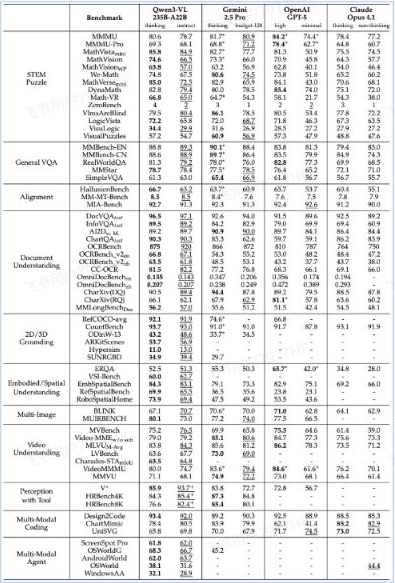
\includegraphics[width=0.98\linewidth,height=0.82\textheight,keepaspectratio]{images/Qwen3-VL/fig-06.png}\end{center}

\end{tcolorbox}
\begin{tcolorbox}[blankest,boxrule=0pt,boxsep=0pt,left=0pt,right=0pt,top=0pt,bottom=0pt]
\begin{center}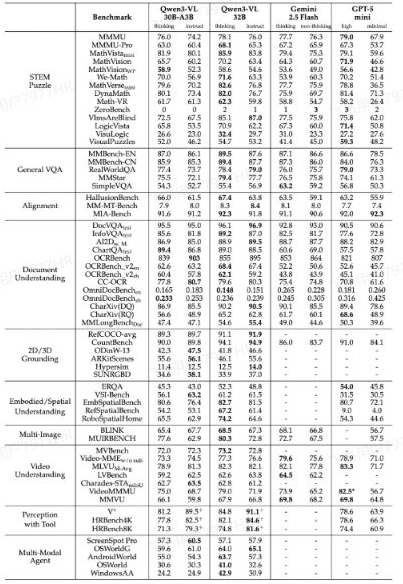
\includegraphics[width=0.98\linewidth,height=0.82\textheight,keepaspectratio]{images/Qwen3-VL/fig-07.png}\end{center}

\end{tcolorbox}
\end{tcbraster}

\textbf{多模态推理}\par

\begin{itemize}[label=\textcolor{feishuBlue}{\textbullet}]
\item 旗舰模型在数学、逻辑等STEM任务（如MathVista、MathVision、ZeroBench）中表现领先，非思考模式（Instruct）和思考模式（Thinking）均优于同类模型。

\end{itemize}

\begin{itemize}[label=\textcolor{feishuBlue}{\textbullet}]
\item 中小型模型（如32B）在复杂推理任务上显著优于前代Qwen2.5-VL-72B，并超越Gemini-2.5-Flash和GPT-5-mini。

\end{itemize}


\end{document}
